\section{優美動作の評価}

\subsection{従来手法}
上田研ではこれまで多くのモデルが提唱されてきた.
その多くは稲津\cite{inazu2}の全曲率計算を起源としている.
先に挙げたB-spline近似で手先軌道を曲線近似し,図\ref{curves}のように
全曲率$\mu$が0.87〜1.31となる曲線を多く含むものを優美としている.
そこから面積や角度に派生するモデルも存在するが,根底は手先軌道である.
今回作成したネットワークが「優美」と判定したものは動画のどの箇所を根拠に
「優美」と判断したのか,動作を抽出して検証する際,どこに着目すべきと
示唆しているかなどを検証した.

\begin{figure}[b]
  \begin{center}
    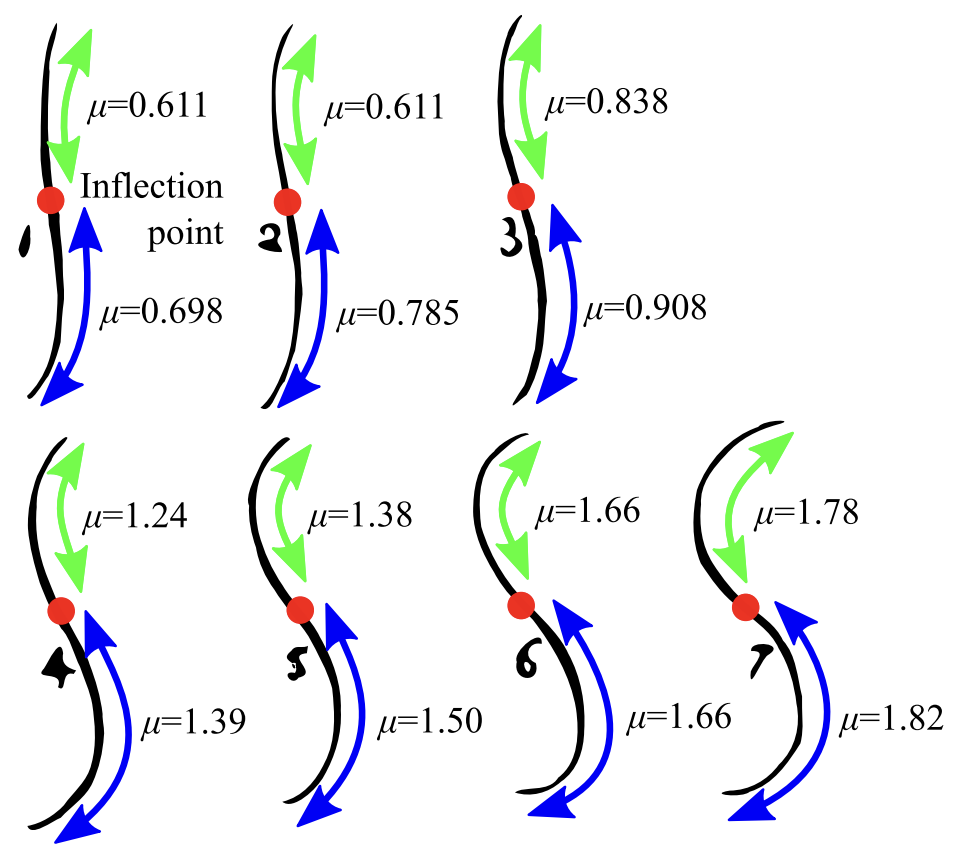
\includegraphics[width=100mm]{images/quote/curves.png}
  \end{center}
  \caption{Hogarth Curveの全曲率}
  \label{curves}
\end{figure}

\subsection{Grad Camを用いた評価}
作成したネットワークの判断根拠を可視化するために,Pytorch-GradCam\cite{pygradcam}を
使用した.作成したネットワークはPytorch\cite{pytorch}でできているので,GradCamも
同じくPytorchでできたものを使用した.

Pytorch-GradCamは入力データに対してどのように各層が影響するか順伝播で確認してから,
逆伝播で影響の強弱を1以下の数値で返す.今回のネットワークでは動画をフレーム毎に区切るので
1フレームずつ処理すると図\ref{camgraph}のように最大30回重複するデータが存在する.
よって出力された結果を順番に足し合わせ,特定のデータについて足し合わされた回数で各値を割ることで
データの均一化を図った.データは1以下にあるので255をかけることでデータの強弱を動画として可視化した.
また,数値は小さいが,データが離散しているので閾値0.4以下の値は0とした.

\begin{figure}[b]
  \begin{center}
    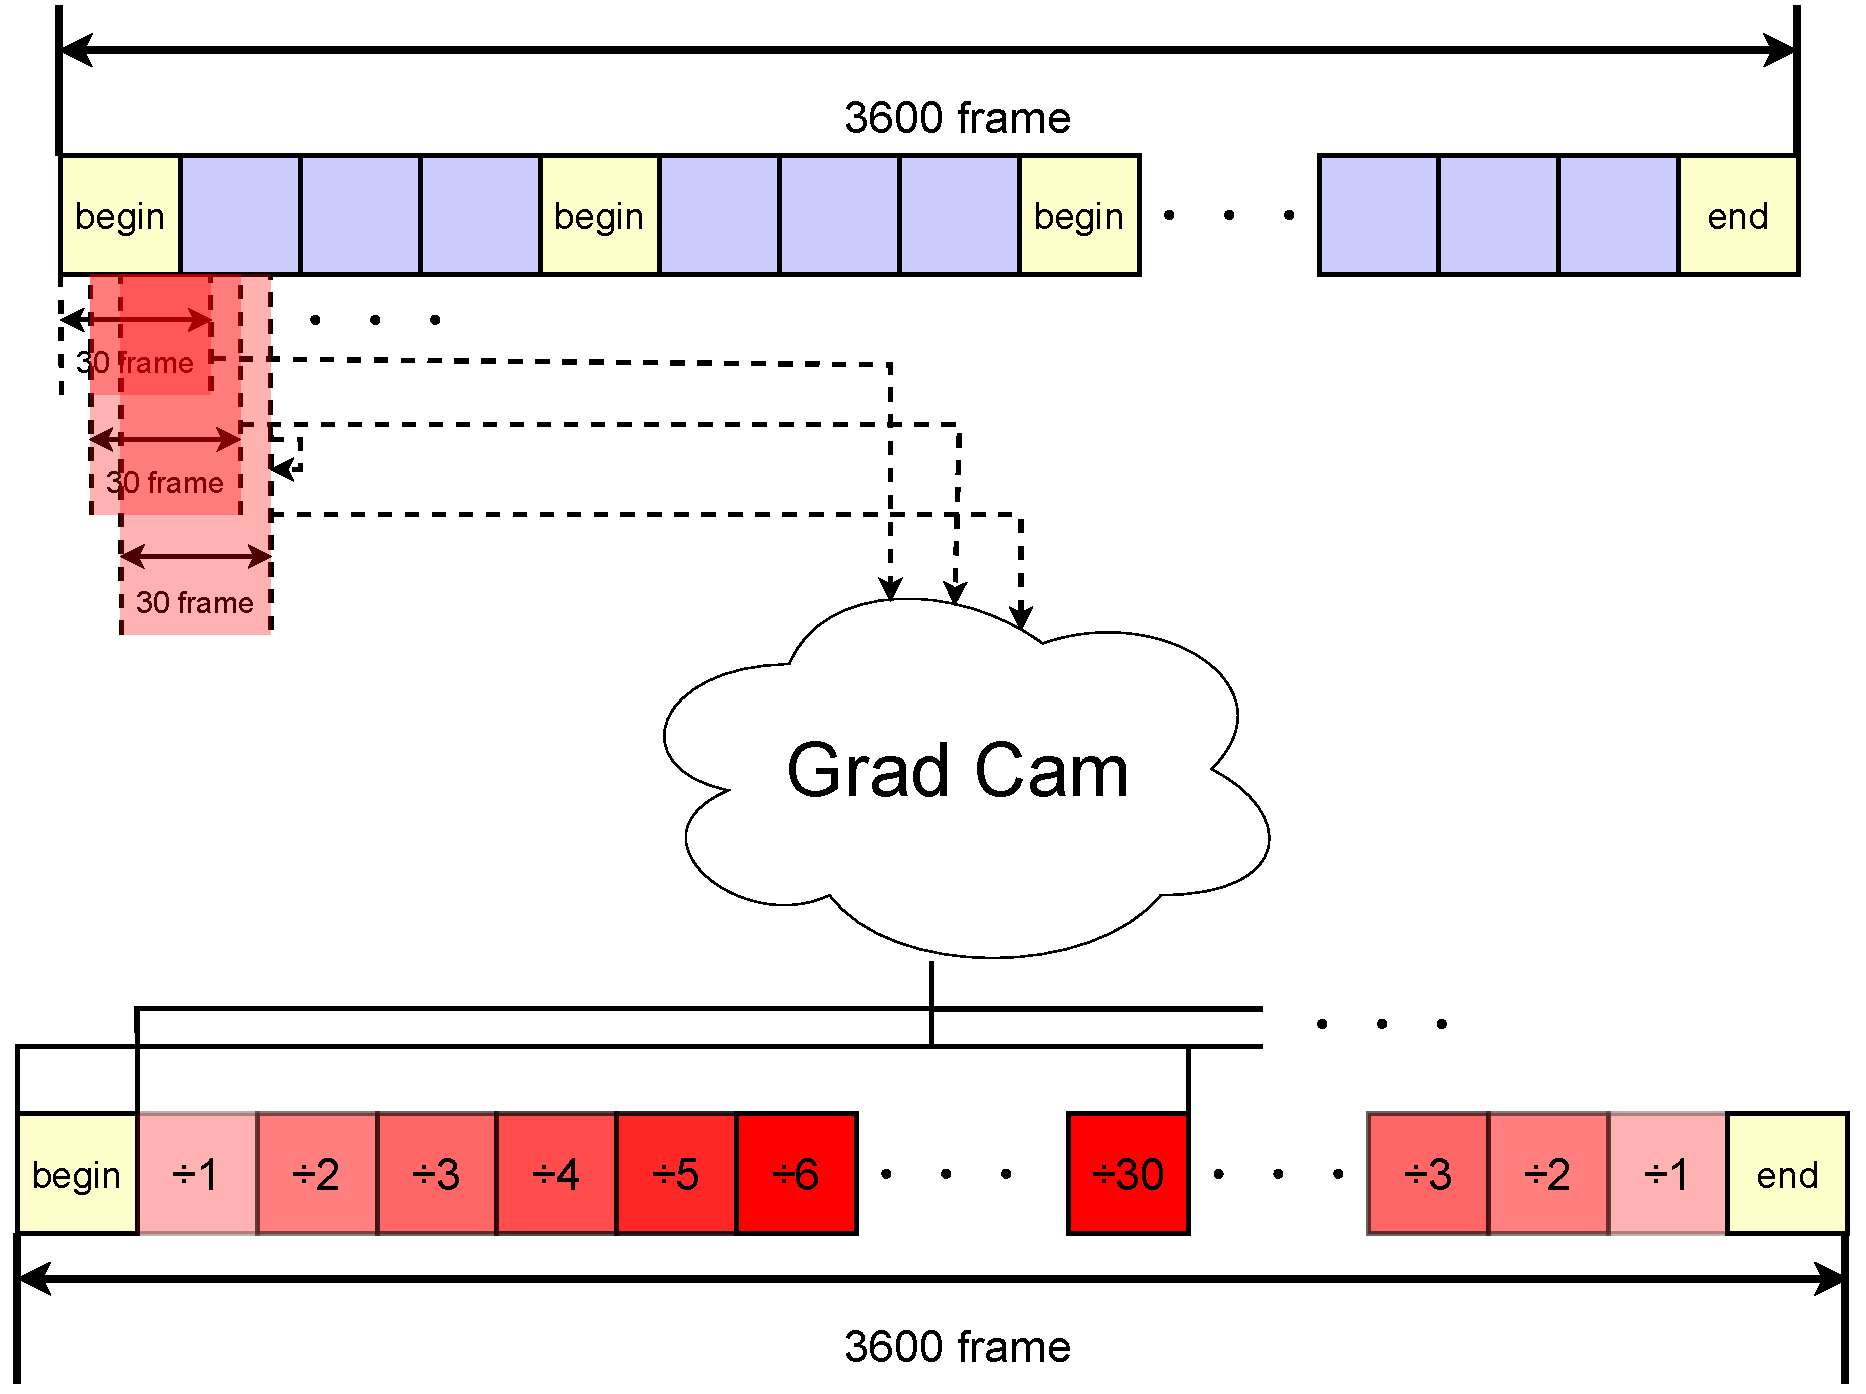
\includegraphics[width=120mm]{images/chart/gradcam.pdf}
  \end{center}
  \caption{Grad Camから出力される結果の整形方法}
  \label{camgraph}
\end{figure}
\clearpage

\begin{table}[t]
  \begin{center}
    \begin{tabular}{|c|cc|} \hline
      優美なダンス
        & 
\includegraphics[width=50mm]{images/cam/chinese.png}
        & 
\includegraphics[width=50mm]{images/cam/japanese.png}
      \\ \hline
      普通のダンス
        & 
\includegraphics[width=50mm]{images/cam/kadokawa.png}
        & 
\includegraphics[width=50mm]{images/cam/aito.png}
      \\ \hline
      その他の動作
        & 
\includegraphics[width=50mm]{images/cam/radio.png}
        & 
\includegraphics[width=50mm]{images/cam/running.png}
      \\ \hline
    \end{tabular}
  \end{center}
  \caption{観測された動画特徴例}
  \label{examples}
\end{table}

このようにして出力されたGrad Camの動画と二値化動画を横に繋ぎ合わせ,どのような特徴があるか
観察した.すると図\ref{examples}のような特徴を観測した.
ここで確率分布は
\begin{enumerate}
  \item 優美なダンスは画面「下部」に「広く」分布している \\
        領域を大きく使っていることから手足を頻繁に使う \\
  \item 普通のダンスは画面「中部」に「小さく」分布している \\
        領域を狭く使っていることから体幹移動を頻繁に使う \\
  \item その他の動作は画面「上部」に「広く」分布している
\end{enumerate}
という仮説を立てた.この仮説を検証するため,それぞれの動画に対して
縦に三つに分割した時の確率分布率を算出した.
\clearpage

\subsection{確率分布を用いた評価}

\subsection{従来手法との比較}